\documentclass[tikz,border=3mm]{standalone}
\usepackage[T1]{fontenc}
\usepackage{lmodern}
\usepackage{amsmath,amssymb}
\usetikzlibrary{arrows.meta,calc,positioning,fit,decorations.pathreplacing}

\definecolor{mistyblue}{HTML}{A3BFD9}
\definecolor{slateblue}{HTML}{7A90B2}
\definecolor{sagegreen}{HTML}{A3BFA3}
\definecolor{dustyteal}{HTML}{6E8B8B}
\definecolor{softgray}{HTML}{D8D8D8}
\definecolor{deepmutedblue}{HTML}{4A5A6A}

% Palette-only aliases used by the existing drawing styles.
\colorlet{navy}{deepmutedblue}
\colorlet{lineblue}{slateblue}
\colorlet{bluefill}{mistyblue!22}
\colorlet{cellblue}{mistyblue!72}
\colorlet{greenline}{dustyteal}
\colorlet{greenfill}{sagegreen!22}
\colorlet{cellgreen}{sagegreen!72}
\colorlet{lavenderline}{slateblue}
\colorlet{lavenderfill}{softgray!55}
\colorlet{brownline}{dustyteal}
\colorlet{brownfill}{softgray!28}
\colorlet{ink}{deepmutedblue}

\begin{document}
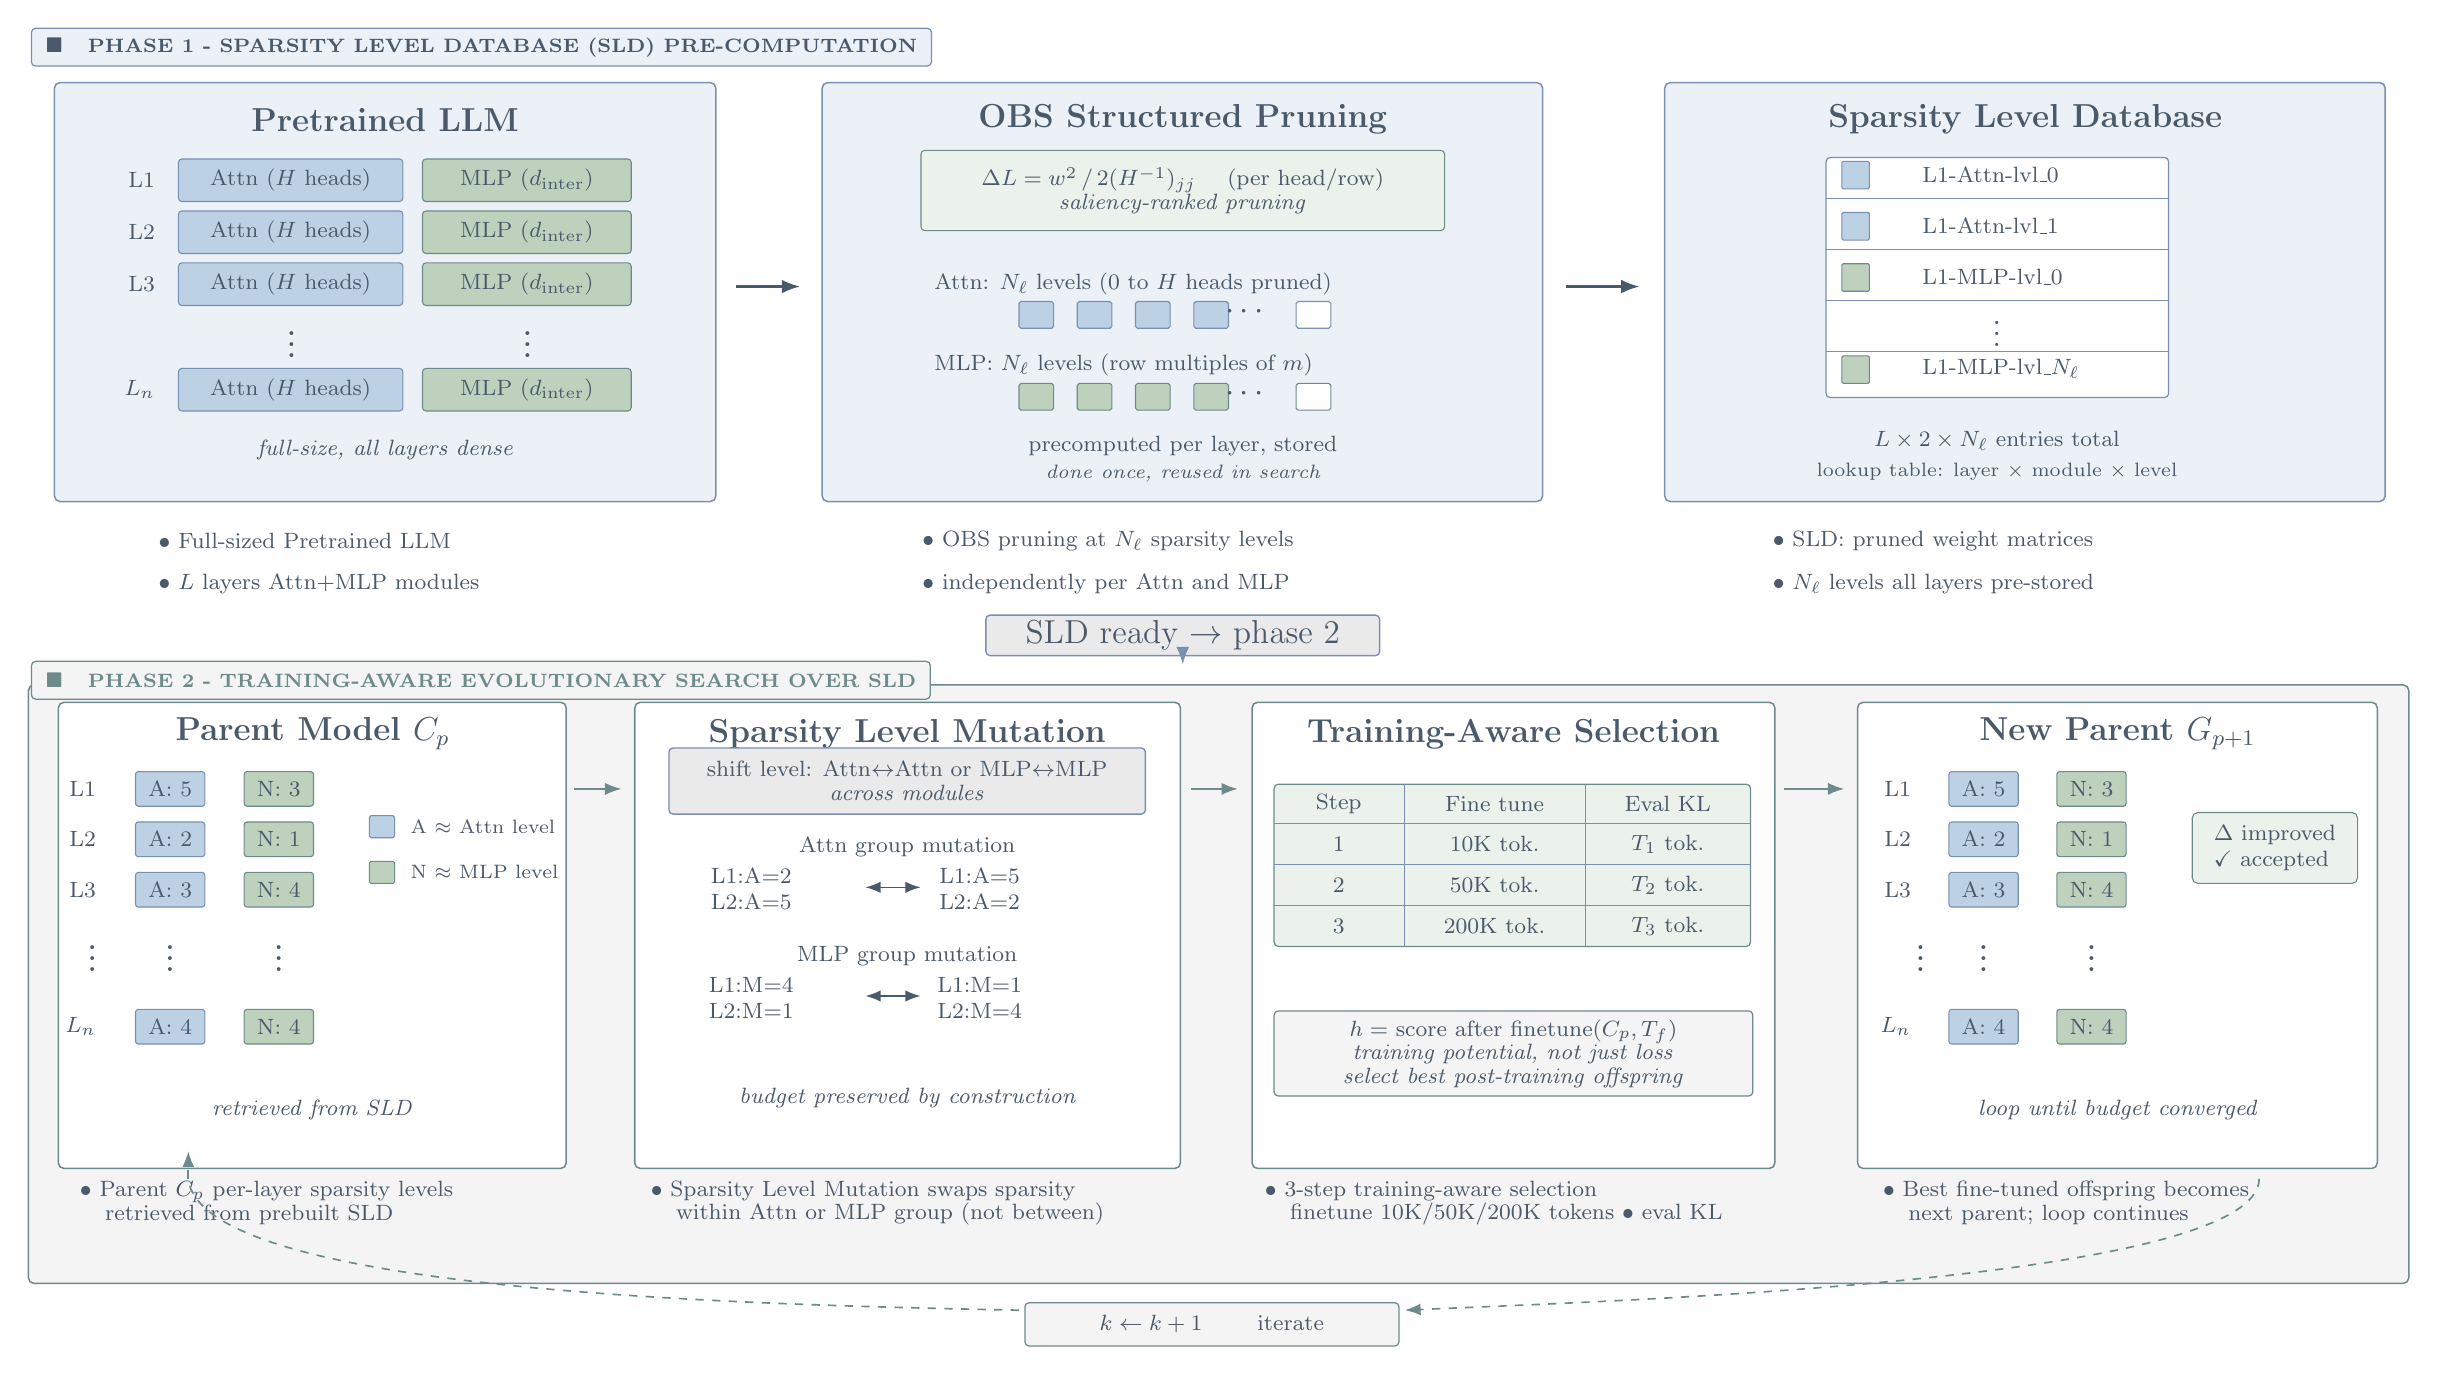
\begin{tikzpicture}[
  x=1cm,y=1cm,
  every node/.style={font=\rmfamily, text=ink, align=center},
  >=Latex,
  panelTop/.style={draw=lineblue, line width=0.55pt, rounded corners=2pt, fill=bluefill},
  panelBot/.style={draw=brownline, line width=0.55pt, rounded corners=2pt, fill=white},
  phaseOne/.style={draw=lineblue, fill=bluefill, rounded corners=1.5pt, line width=0.45pt, inner xsep=0.18cm, inner ysep=0.07cm},
  phaseTwo/.style={draw=brownline, fill=brownfill, rounded corners=1.5pt, line width=0.45pt, inner xsep=0.18cm, inner ysep=0.07cm},
  title/.style={font=\rmfamily\bfseries\large, text=navy, align=center},
  btitle/.style={font=\rmfamily\bfseries\large, text=deepmutedblue, align=center},
  tinytext/.style={font=\rmfamily\scriptsize, align=center},
  smalltext/.style={font=\rmfamily\footnotesize, align=center},
  moduleBlue/.style={draw=lineblue, fill=cellblue, rounded corners=1.2pt, minimum width=2.85cm, minimum height=0.54cm, inner sep=0.02cm, font=\rmfamily\footnotesize},
  moduleGreen/.style={draw=greenline, fill=cellgreen, rounded corners=1.2pt, minimum width=2.65cm, minimum height=0.54cm, inner sep=0.02cm, font=\rmfamily\footnotesize},
  smallA/.style={draw=lineblue, fill=cellblue, rounded corners=1pt, minimum width=0.88cm, minimum height=0.44cm, inner sep=0pt, font=\rmfamily\footnotesize},
  smallN/.style={draw=greenline, fill=cellgreen, rounded corners=1pt, minimum width=0.88cm, minimum height=0.44cm, inner sep=0pt, font=\rmfamily\footnotesize},
  noteBox/.style={draw=lavenderline, fill=lavenderfill, rounded corners=1.5pt, line width=0.5pt, inner sep=0.07cm, font=\rmfamily\footnotesize},
  scoreBox/.style={draw=brownline, fill=brownfill, rounded corners=1.5pt, line width=0.45pt, inner sep=0.06cm, font=\rmfamily\footnotesize}
]

% ----------------------------------------------------------------------
% Phase 1 title
% ----------------------------------------------------------------------
\node[phaseOne, anchor=west, font=\rmfamily\bfseries\large, text=navy, minimum height=0.48cm]
  at (0.05,16.37) {\scriptsize$\blacksquare$\quad PHASE 1 - SPARSITY LEVEL DATABASE (SLD) PRE-COMPUTATION};

% ----------------------------------------------------------------------
% Phase 1 panels
% ----------------------------------------------------------------------
\draw[panelTop] (0.35,10.60) rectangle (8.75,15.92);
\draw[panelTop] (10.10,10.60) rectangle (19.25,15.92);
\draw[panelTop] (20.80,10.60) rectangle (29.95,15.92);

\node[title] at (4.55,15.45) {Pretrained LLM};
\node[title] at (14.68,15.45) {OBS Structured Pruning};
\node[title] at (25.38,15.45) {Sparsity Level Database};

% Panel 1: pretrained LLM
\foreach \y/\lab/\av/\nv in {14.68/L1/{Attn ($H$ heads)}/{MLP ($d_{\mathrm{inter}}$)},14.02/L2/{Attn ($H$ heads)}/{MLP ($d_{\mathrm{inter}}$)},13.36/L3/{Attn ($H$ heads)}/{MLP ($d_{\mathrm{inter}}$)},12.02/$L_n$/{Attn ($H$ heads)}/{MLP ($d_{\mathrm{inter}}$)}}{
  \node[smalltext, anchor=east] at (1.75,\y) {\lab};
  \node[moduleBlue] at (3.35,\y) {\av};
  \node[moduleGreen] at (6.35,\y) {\nv};
}
\node[font=\rmfamily\Large] at (3.36,12.70) {$\vdots$};
\node[font=\rmfamily\Large] at (6.36,12.70) {$\vdots$};
\node[font=\rmfamily\itshape\footnotesize] at (4.55,11.25) {full-size, all layers dense};

\node[anchor=west, font=\rmfamily\footnotesize, align=left] at (1.55,10.10) {$\bullet$ Full-sized Pretrained LLM};
\node[anchor=west, font=\rmfamily\footnotesize, align=left] at (1.55,9.55) {$\bullet$ $L$ layers Attn+MLP modules};

% arrows between phase 1 panels
\draw[->, line width=0.8pt, draw=navy] (9.00,13.33) -- (9.82,13.33);
\draw[->, line width=0.8pt, draw=navy] (19.55,13.33) -- (20.48,13.33);

% Panel 2: OBS structured pruning
\node[draw=greenline, fill=greenfill, rounded corners=1.4pt, minimum width=6.65cm, minimum height=1.02cm, font=\rmfamily\footnotesize] at (14.68,14.55)
  {$\Delta L = w^2\,/\,2(H^{-1})_{jj}$ \quad (per head/row)\\[-1pt]
   \textit{saliency-ranked pruning}};
\node[anchor=west, font=\rmfamily\footnotesize, align=left] at (11.40,13.36) {Attn: $N_\ell$ levels (0 to $H$ heads pruned)};
\foreach \x/\c in {12.60/cellblue,13.34/cellblue,14.08/cellblue,14.82/cellblue,16.12/white}{
  \draw[draw=lineblue, fill=\c, rounded corners=0.7pt] (\x,12.80) rectangle +(0.44,0.34);
}
\node[font=\rmfamily\large] at (15.50,13.00) {$\cdots$};
\node[anchor=west, font=\rmfamily\footnotesize, align=left] at (11.40,12.33) {MLP: $N_\ell$ levels (row multiples of $m$)};
\foreach \x/\c in {12.60/cellgreen,13.34/cellgreen,14.08/cellgreen,14.82/cellgreen,16.12/white}{
  \draw[draw=greenline, fill=\c, rounded corners=0.7pt] (\x,11.76) rectangle +(0.44,0.34);
}
\node[font=\rmfamily\large] at (15.50,11.96) {$\cdots$};
\node[font=\rmfamily\footnotesize] at (14.68,11.30) {precomputed per layer, stored};
\node[font=\rmfamily\itshape\scriptsize, text=navy] at (14.68,10.96) {done once, reused in search};

\node[anchor=west, font=\rmfamily\footnotesize, align=left] at (11.25,10.10) {$\bullet$ OBS pruning at $N_\ell$ sparsity levels};
\node[anchor=west, font=\rmfamily\footnotesize, align=left] at (11.25,9.55) {$\bullet$ independently per Attn and MLP};


% Panel 3: database
\begin{scope}[shift={(22.85,11.92)}]
  \draw[draw=slateblue, fill=white, rounded corners=1.5pt, line width=0.45pt] (0,0) rectangle (4.35,3.05);
  \foreach \yy in {0.58,1.23,1.88,2.53}{\draw[slateblue, line width=0.35pt] (0,\yy) -- (4.35,\yy);}
  \draw[draw=lineblue, fill=cellblue, rounded corners=0.5pt] (0.20,2.65) rectangle (0.55,3.00);
  \node[anchor=west, font=\rmfamily\footnotesize] at (1.10,2.83) {L1-Attn-lvl\_0};
  \draw[draw=lineblue, fill=cellblue, rounded corners=0.5pt] (0.20,2.00) rectangle (0.55,2.35);
  \node[anchor=west, font=\rmfamily\footnotesize] at (1.10,2.18) {L1-Attn-lvl\_1};
  \draw[draw=greenline, fill=cellgreen, rounded corners=0.5pt] (0.20,1.35) rectangle (0.55,1.70);
  \node[anchor=west, font=\rmfamily\footnotesize] at (1.10,1.53) {L1-MLP-lvl\_0};
  \node[font=\rmfamily\large] at (2.17,0.91) {$\vdots$};
  \draw[draw=greenline, fill=cellgreen, rounded corners=0.5pt] (0.20,0.18) rectangle (0.55,0.53);
  \node[anchor=west, font=\rmfamily\footnotesize] at (1.10,0.36) {L1-MLP-lvl\_$N_\ell$};
\end{scope}
\node[font=\rmfamily\footnotesize] at (25.02,11.37) {$L\times 2\times N_\ell$ entries total};
\node[font=\rmfamily\scriptsize] at (25.02,10.98) {lookup table: layer $\times$ module $\times$ level};

\node[anchor=west, font=\rmfamily\footnotesize, align=left] at (22.05,10.10) {$\bullet$ SLD: pruned weight matrices};
\node[anchor=west, font=\rmfamily\footnotesize, align=left] at (22.05,9.55) {$\bullet$ $N_\ell$ levels all layers pre-stored};

% ----------------------------------------------------------------------
% Phase 2 background and title
% ----------------------------------------------------------------------
\begin{scope}[yshift=-0.65cm]
\draw[draw=brownline, fill=brownfill, rounded corners=2pt, line width=0.55pt] (0.02,1.32) rectangle (30.25,8.92);
\node[phaseTwo, anchor=west, font=\rmfamily\bfseries\large, text=brownline, minimum height=0.48cm]
  at (0.05,8.98) {\scriptsize$\blacksquare$\quad PHASE 2 - TRAINING-AWARE EVOLUTIONARY SEARCH OVER SLD};


% Phase 2 panels
\draw[panelBot] (0.40,2.78) rectangle (6.85,8.70);
\draw[panelBot] (7.72,2.78) rectangle (14.65,8.70);
\draw[panelBot] (15.56,2.78) rectangle (22.20,8.70);
\draw[panelBot] (23.25,2.78) rectangle (29.85,8.70);

\node[btitle] at (3.63,8.30) {Parent Model $C_p$};
\node[btitle] at (11.18,8.30) {Sparsity Level Mutation};
\node[btitle] at (18.88,8.30) {Training-Aware Selection};
\node[btitle] at (26.55,8.30) {New Parent $G_{p+1}$};

% Bottom arrows between panels
\draw[->, line width=0.65pt, draw=brownline] (6.95,7.60) -- (7.55,7.60);
\draw[->, line width=0.65pt, draw=brownline] (14.78,7.60) -- (15.38,7.60);
\draw[->, line width=0.65pt, draw=brownline] (22.32,7.60) -- (23.08,7.60);

% Parent model panel
\foreach \y/\lab/\a/\n in {7.60/L1/5/3,6.96/L2/2/1,6.32/L3/3/4,4.58/$L_n$/4/4}{
  \node[smalltext, anchor=east] at (1.00,\y) {\lab};
  \node[smallA] at (1.82,\y) {A: \a};
  \node[smallN] at (3.20,\y) {N: \n};
}
\node[font=\rmfamily\Large] at (1.82,5.55) {$\vdots$};
\node[font=\rmfamily\Large] at (3.20,5.55) {$\vdots$};
\node[font=\rmfamily\Large] at (0.83,5.55) {$\vdots$};
\draw[draw=lineblue, fill=cellblue, rounded corners=0.6pt] (4.35,6.98) rectangle +(0.32,0.28);
\node[anchor=west, font=\rmfamily\scriptsize] at (4.75,7.12) {A $\approx$ Attn level};
\draw[draw=greenline, fill=cellgreen, rounded corners=0.6pt] (4.35,6.40) rectangle +(0.32,0.28);
\node[anchor=west, font=\rmfamily\scriptsize] at (4.75,6.54) {N $\approx$ MLP level};
\node[font=\rmfamily\itshape\footnotesize] at (3.62,3.52) {retrieved from SLD};
\node[anchor=west, font=\rmfamily\footnotesize, align=left] at (0.55,2.34)
  {$\bullet$ Parent $C_p$ per-layer sparsity levels\\[-1pt]\hspace{0.32cm}retrieved from prebuilt SLD};

% Mutation panel
\node[noteBox, minimum width=6.05cm, minimum height=0.84cm] at (11.18,7.70)
  {shift level: Attn$\leftrightarrow$Attn or MLP$\leftrightarrow$MLP\\[-1pt]
   \textit{across modules}};
\node[font=\rmfamily\footnotesize] at (11.18,6.86) {Attn group mutation};
\node[font=\rmfamily\footnotesize, align=left] at (9.20,6.33) {L1:A=2\\L2:A=5};
\node[font=\rmfamily\footnotesize, align=left] at (12.10,6.33) {L1:A=5\\L2:A=2};
\draw[<->, draw=deepmutedblue, line width=0.55pt] (10.65,6.35) -- (11.35,6.35);
\node[font=\rmfamily\footnotesize] at (11.18,5.48) {MLP group mutation};
\node[font=\rmfamily\footnotesize, align=left] at (9.20,4.95) {L1:M=4\\L2:M=1};
\node[font=\rmfamily\footnotesize, align=left] at (12.10,4.95) {L1:M=1\\L2:M=4};
\draw[<->, draw=deepmutedblue, line width=0.55pt] (10.65,4.97) -- (11.35,4.97);
\node[font=\rmfamily\itshape\footnotesize] at (11.18,3.68) {budget preserved by construction};
\node[anchor=west, font=\rmfamily\footnotesize, align=left] at (7.80,2.34)
  {$\bullet$ Sparsity Level Mutation swaps sparsity\\[-1pt]\hspace{0.32cm}within Attn or MLP group (not between)};

% Selection panel table
\begin{scope}[shift={(15.84,5.60)}]
  \draw[draw=greenline, fill=greenfill, rounded corners=1.5pt, line width=0.45pt] (0,0) rectangle (6.05,2.06);
  \foreach \x in {1.65,3.95}{\draw[slateblue, line width=0.35pt] (\x,0) -- (\x,2.06);}
  \foreach \y in {0.52,1.04,1.56}{\draw[slateblue, line width=0.35pt] (0,\y) -- (6.05,\y);}
  \node[font=\rmfamily\footnotesize] at (0.82,1.81) {Step};
  \node[font=\rmfamily\footnotesize] at (2.80,1.81) {Fine tune};
  \node[font=\rmfamily\footnotesize] at (5.00,1.81) {Eval KL};
  \node[font=\rmfamily\footnotesize] at (0.82,1.30) {1};
  \node[font=\rmfamily\footnotesize] at (2.80,1.30) {10K tok.};
  \node[font=\rmfamily\footnotesize] at (5.00,1.30) {$T_1$ tok.};
  \node[font=\rmfamily\footnotesize] at (0.82,0.78) {2};
  \node[font=\rmfamily\footnotesize] at (2.80,0.78) {50K tok.};
  \node[font=\rmfamily\footnotesize] at (5.00,0.78) {$T_2$ tok.};
  \node[font=\rmfamily\footnotesize] at (0.82,0.26) {3};
  \node[font=\rmfamily\footnotesize] at (2.80,0.26) {200K tok.};
  \node[font=\rmfamily\footnotesize] at (5.00,0.26) {$T_3$ tok.};
\end{scope}
\node[scoreBox, minimum width=6.08cm, minimum height=1.08cm] at (18.88,4.24)
  {$h =$ score after finetune$(C_p,T_f)$\\[-1pt]
   \textit{training potential, not just loss}\\[-1pt]
   \textit{select best post-training offspring}};
\node[anchor=west, font=\rmfamily\footnotesize, align=left] at (15.60,2.34)
  {$\bullet$ 3-step training-aware selection\\[-1pt]\hspace{0.32cm}finetune 10K/50K/200K tokens $\bullet$ eval KL};

% New parent panel
\foreach \y/\lab/\a/\n in {7.60/L1/5/3,6.96/L2/2/1,6.32/L3/3/4,4.58/$L_n$/4/4}{
  \node[smalltext, anchor=east] at (24.05,\y) {\lab};
  \node[smallA] at (24.85,\y) {A: \a};
  \node[smallN] at (26.22,\y) {N: \n};
}
\node[font=\rmfamily\Large] at (24.85,5.55) {$\vdots$};
\node[font=\rmfamily\Large] at (26.22,5.55) {$\vdots$};
\node[font=\rmfamily\Large] at (24.05,5.55) {$\vdots$};
\node[draw=greenline, fill=greenfill, rounded corners=2pt, minimum width=2.10cm, minimum height=0.90cm, font=\rmfamily\footnotesize, align=left] at (28.55,6.85)
  {$\Delta$ improved\\$\checkmark$ accepted};
\node[font=\rmfamily\itshape\footnotesize] at (26.55,3.52) {loop until budget converged};
\node[anchor=west, font=\rmfamily\footnotesize, align=left] at (23.45,2.34)
  {$\bullet$ Best fine-tuned offspring becomes\\[-1pt]\hspace{0.32cm}next parent; loop continues};

% ----------------------------------------------------------------------
% Iteration loop
% ----------------------------------------------------------------------
\node[scoreBox, minimum width=4.75cm, minimum height=0.55cm, font=\rmfamily\footnotesize] (iter) at (15.05,0.80) {$k \leftarrow k+1$ \qquad iterate};
\draw[->, draw=brownline, line width=0.60pt, dashed]
  (28.35,2.65) .. controls (28.35,1.35) and (20.20,1.10) .. (17.50,0.98);
\draw[draw=brownline, line width=0.60pt, dashed]
  (12.60,0.98) .. controls (9.20,1.05) and (2.20,1.20) .. (2.05,2.65);
\draw[->, draw=brownline, line width=0.60pt, dashed]
  (2.05,2.65) -- (2.05,3.00);


\end{scope}

% Handoff note intentionally drawn last so it is not hidden by the Phase 2 band.
\node[noteBox, minimum width=5.00cm, minimum height=0.50cm, text=navy, font=\rmfamily\large] at (14.68,8.90) {SLD ready $\rightarrow$ phase 2};
\draw[->, draw=lavenderline, line width=0.75pt] (14.68,8.60) -- (14.68,8.53);

\end{tikzpicture}
\end{document}
